\documentclass[a4paper]{article}
\usepackage[utf8]{inputenc}
\usepackage[T1]{fontenc}
\usepackage[ngerman]{babel}
\usepackage{lmodern, amsmath, amssymb, graphicx, parskip}
\usepackage[round]{natbib}

\begin{document}

\title{Ergebnisse der Besprechung vom 3. April 2014}
\date{}
\author{Ullika Scholz}
\maketitle
\thispagestyle{empty}
\setlength{\parskip}{6pt}

Meine Bachelorarbeit wird aus zwei Teilen bestehen. Das Thema sind weiterhin Moiré-Effekte beim Domain-Coloring (siehe Proposal vom 26.2.). Im ersten Teil werde ich einen Entscheidungsautomaten entwickeln, der zu gegebener Funktion $h^*: \mathbb{C} \rightarrow \mathbb{C}$ und gegebenen Pixel-Auflösungen $res_x$ und $res_y$ entscheidet, ob die Funktion angemessen darstellbar ist. Im zweiten Teil soll, falls dafür noch Zeit ist, die Entstehung der Wellenmuster erklärt werden.

In der Besprechung vom 3. April ging es nur um den ersten Teil, also um die Entwicklung des Automaten. Um die Sache zu vereinfachen, nehme ich in dieser Übersicht an, dass es sich bei $h^*$ um eine Funktion auf $\mathbb{R}$ handelt und wir nur die Auflösung in x-Richtung $res_x$ betrachten müssen.

Bislang steht fest \cite[vgl.][]{MuellerWichards1999}:

\textit{Für jede abschnittsweise stetige Funktion $h(t)$ auf einem Intervall $[a,b]$ existiert eine Darstellung als Fourier-Reihe, also:}
$$h(t)=\lim\limits_{n \rightarrow \infty} f_n(h)(t) \text{, wobei}$$
$$f_n(h)(t)=\sum\limits_{-n}^{n} c_n e^{in \omega t}.$$
Die Koeffizienten $c_n \in \mathbb{C}$ werden dabei u.a. aus dem Integral der Funktion $h$ berechnet.

Falls die Funktion $h^*$ aus dem Raum $\mathcal{F}=\{h \in C[a,b]: h \equiv f_{res_x}(h) \}$, also aus dem Raum derjenigen Funktionen stammt, deren Fourier-Reihenentwicklung bei $n=res_x$ abbricht, ist die Sache klar. Denn dann ist $h^*$ mit $res_x$ bandbegrenzt und folgender Satz kann unmittelbar angewendet werden:

\textbf{Satz (Abtasttheorem)} \cite[nach][]{MuellerWichards1999}

\textit{Ein Zeitsignal $x(t)$, das mit $f_g$ bandbegrenzt ist und mit einer Abtastfrequenz $1/T_a \geq 2 f_g$ abgetastet wird, kann aus dem Abtastsignal [...] fehlerfrei wiedergewonnen werden.}

Wir können also unseren Automaten ein sicheres "`Ja"'  ausgeben lassen.

Die meisten Funktionen wie z.B. Polynome haben allerdings eine Fourier-Rei\-henentwicklung, die nie abbricht. Trotzdem lassen sich viele dieser Funktionen weitgehend fehlerfrei darstellen. Angenommen $h^*$ ist so eine Funktion. Was soll der Entscheidungsautomat  machen?

Idee: Wir suchen im Funktionenraum $\mathcal{F}$ nach derjenigen korrekt darstellbaren Funktion $f^*$, die sich von unserer Funktion $h^*$ am wenigsten unterscheidet. Je nachdem, ob der Fehler $\varepsilon=\lVert h^*-f^*\rVert_{\infty}$ groß oder klein ist, entscheiden wir, ob wir die Funktion $h^*$ akzeptieren.
Diese Vorgehensweise soll zur Folge haben, dass wir Funktionen, deren Frequenzanteile ab $res_x$ gering sind, akzeptieren (Abb.\ref{Abb.1}), während wir Funktionen, bei denen gerade diese Frequenzen eine Rolle spielen, ablehnen (Abb.\ref{Abb.2}).

In diesem Beispiel wurden für $h^*$ zwei verschiedene reelle Polynome auf dem Intervall $[-1,1]$ und eine Auflösung von 2,5 Pixeln pro Einheit gewählt.

\begin{figure}[ht]
\centering
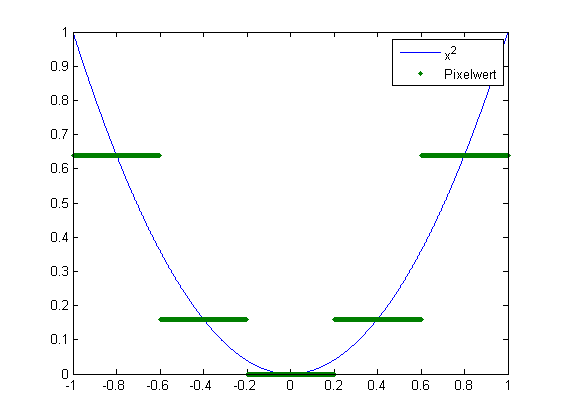
\includegraphics[width=0.5\textwidth]{parabelplot.png}
\caption{Abtastung einer Parabel}
\label{Abb.1}
\end{figure}
\begin{figure}[ht]
\centering
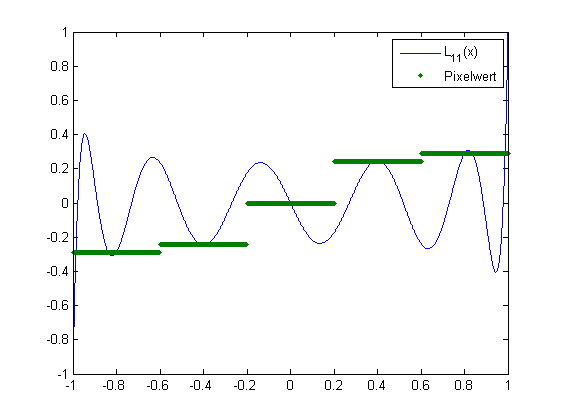
\includegraphics[width=0.5\textwidth]{legendre11plot.png}
\caption{Abtastung des elften Legendre-Polynoms}
\label{Abb.2}
\end{figure}

Warum $\varepsilon=\lVert h^*-f^*\rVert_{\infty}$ in Abb.\ref{Abb.2} nicht bloß zufällig größer als in Abb.\ref{Abb.1} ist, werde ich in den nächsten Wochen ebenso zeigen, wie dass es sich bei der Funktion $f^*$ um $f_{res_x}(h^*)$ handelt, also um die Reihenentwicklung von $h^*$, die nach $res_x$ Gliedern abgeschnitten wird.

Weitere Literatur: \cite[]{Achilles1978} sowie \cite[]{Schroeder1978}.

\bibliography{lit}
\bibliographystyle{alpha}

\end{document}





